\documentclass[aspectratio=169]{beamer}

\usetheme{Rochester}
\usecolortheme{default}
\setbeamertemplate{navigation symbols}{}

\usepackage{iftex}
\ifPDFTeX
  \usepackage[T1]{fontenc}
  \usepackage[utf8]{inputenc}
\else
  \usepackage{fontspec}
\fi
\usepackage{booktabs}
\usepackage{amsmath}
\usepackage{graphicx}
\usepackage{tikz}
\usetikzlibrary{arrows.meta,positioning,shapes.geometric,fit,calc}

\title[PathMNIST Cancer Detection]{Improving Cancer-Related Tissue Classification\\ \large with Expert-Based Correction}
\subtitle{PathMNIST Classification Improvement}
\author{Nick Zerjeski}
\institute{Free University of Bozen-Bolzano}
\date{\today}

\tikzset{
  modelblock/.style={draw, rounded corners=2pt, align=center, minimum width=2.6cm, minimum height=0.8cm, fill=blue!8},
  expertblock/.style={draw, rounded corners=2pt, align=center, minimum width=2.8cm, minimum height=0.8cm, fill=green!10},
  decisionblock/.style={draw, diamond, aspect=2.1, align=center, inner sep=1pt, fill=orange!12},
  arrow/.style={-{Latex[length=2.4mm]}, thick},
  weakarrow/.style={-{Latex[length=2.4mm]}, thick, dashed, gray!60}
}

\begin{document}

\begin{frame}
  \titlepage
\end{frame}

\begin{frame}{Overview}
  \tableofcontents
\end{frame}

\section{Motivation and Dataset}

\begin{frame}{Motivation}
  \begin{itemize}
    \item<1-> Histopathological analysis is central for cancer diagnosis.
    \item<2-> Manual image analysis is time-consuming and depends on expert judgement.
    \item<3-> In medical classification, false negatives for cancer-related tissue are especially costly.
    \item<4-> The goal is therefore recall-oriented improvement, not only higher accuracy.
  \end{itemize}
  \begin{block}<5->{Project Question}
    Can targeted binary expert classifiers correct the main weaknesses of a general PathMNIST classifier?
  \end{block}
\end{frame}

\begin{frame}{PathMNIST Dataset}
  \begin{columns}[T,onlytextwidth]
    \begin{column}{0.44\textwidth}
      \begin{itemize}
        \item 107,180 colorectal cancer histology patches.
        \item Splits: 89,996 train, 10,004 validation, 7,180 test.
        \item Nine tissue classes.
        \item Images available at $28 \times 28$ and $224 \times 224$ pixels.
      \end{itemize}
      \begin{block}{Cancer-related classes}
        Cancer-associated stroma and colorectal adenocarcinoma epithelium.
      \end{block}
    \end{column}
    \begin{column}{0.54\textwidth}
      \centering
      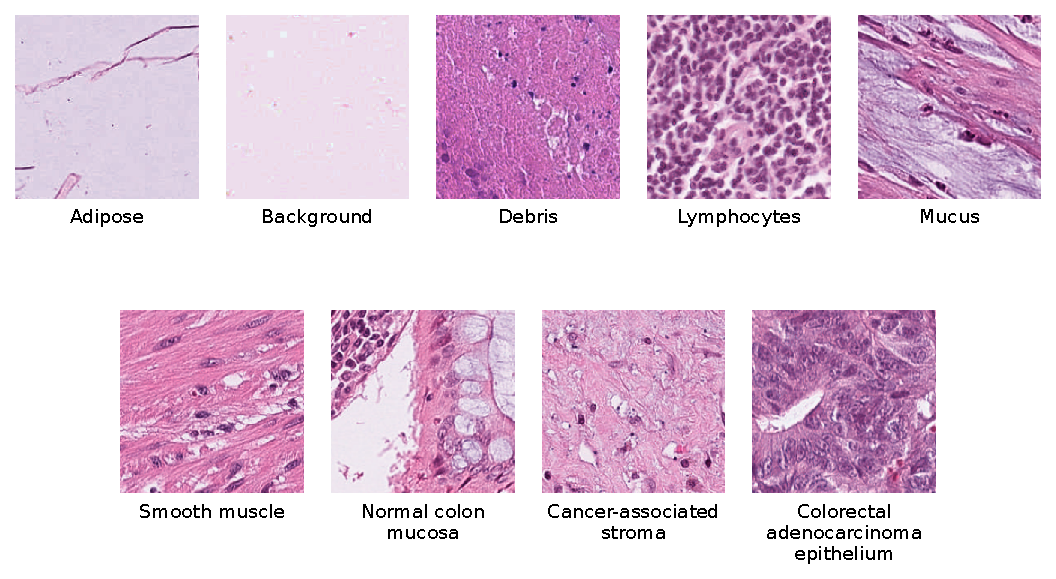
\includegraphics[width=\textwidth]{figures/pathmnist_class_examples}
    \end{column}
  \end{columns}
\end{frame}

\begin{frame}{Class Distribution}
  \centering
  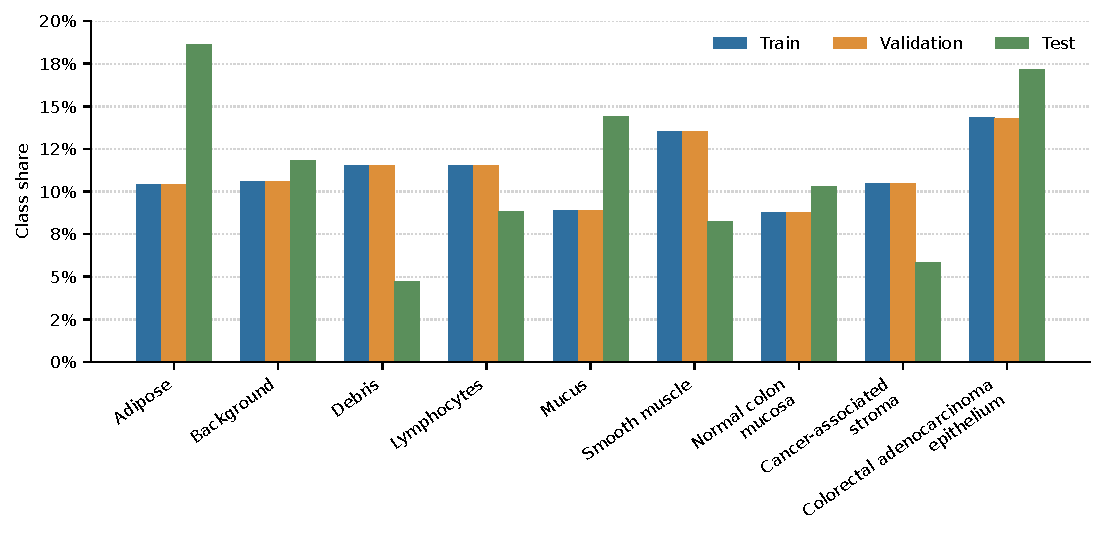
\includegraphics[width=0.82\textwidth]{figures/pathmnist_class_distribution}
  \vspace{0.4em}
  \begin{itemize}
    \item Smooth muscle and epithelium are among the largest class fractions.
    \item Stroma is clinically relevant but harder for the baseline model.
  \end{itemize}
\end{frame}

\section{Model Development}

\begin{frame}{Reference and Base Model}
  \begin{columns}[T,onlytextwidth]
    \begin{column}{0.48\textwidth}
      \begin{block}{External reference}
        Official MedMNIST ResNet-50 benchmark at $28 \times 28$ resolution.
      \end{block}
      \begin{itemize}
        \item Strong overall benchmark.
        \item Used as an external comparison point.
      \end{itemize}
    \end{column}
    \begin{column}{0.48\textwidth}
      \begin{block}{Base model}
        Custom CNN trained from scratch on $224 \times 224$ PathMNIST.
      \end{block}
      \begin{itemize}
        \item 5 convolutional layers.
        \item Batch normalization and SiLU activations.
        \item 558,921 trainable parameters.
      \end{itemize}
    \end{column}
  \end{columns}
\end{frame}

\begin{frame}{Base CNN Architecture}
  \centering
  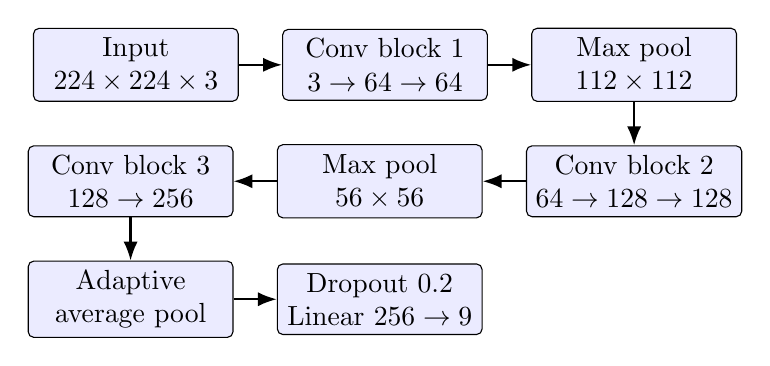
\begin{tikzpicture}[node distance=0.55cm]
    \node[modelblock] (input) {Input\\$224 \times 224 \times 3$};
    \node[modelblock, right=of input] (conv1) {Conv block 1\\$3 \rightarrow 64 \rightarrow 64$};
    \node[modelblock, right=of conv1] (pool1) {Max pool\\$112 \times 112$};
    \node[modelblock, below=of pool1] (conv2) {Conv block 2\\$64 \rightarrow 128 \rightarrow 128$};
    \node[modelblock, left=of conv2] (pool2) {Max pool\\$56 \times 56$};
    \node[modelblock, left=of pool2] (conv3) {Conv block 3\\$128 \rightarrow 256$};
    \node[modelblock, below=of conv3] (gap) {Adaptive\\average pool};
    \node[modelblock, right=of gap] (head) {Dropout $0.2$\\Linear $256 \rightarrow 9$};

    \draw[arrow] (input) -- (conv1);
    \draw[arrow] (conv1) -- (pool1);
    \draw[arrow] (pool1) -- (conv2);
    \draw[arrow] (conv2) -- (pool2);
    \draw[arrow] (pool2) -- (conv3);
    \draw[arrow] (conv3) -- (gap);
    \draw[arrow] (gap) -- (head);
  \end{tikzpicture}
  \vspace{0.5em}
  \begin{itemize}
    \item Trained for 10 epochs with AdamW, cosine learning-rate schedule, histology augmentation, label smoothing, and mixup.
  \end{itemize}
\end{frame}

\begin{frame}{Base Model Performance}
  \begin{columns}[T,onlytextwidth]
    \begin{column}{0.50\textwidth}
      \begin{itemize}
        \item Overall accuracy: $0.906$.
        \item Overall $F_2$: $0.885$.
        \item Epithelium recall: $0.989$.
        \item Stroma recall: only $0.520$.
      \end{itemize}
      \begin{block}{Main weakness}
        Stroma is repeatedly confused with debris, smooth muscle, and epithelium.
      \end{block}
    \end{column}
    \begin{column}{0.48\textwidth}
      \centering
      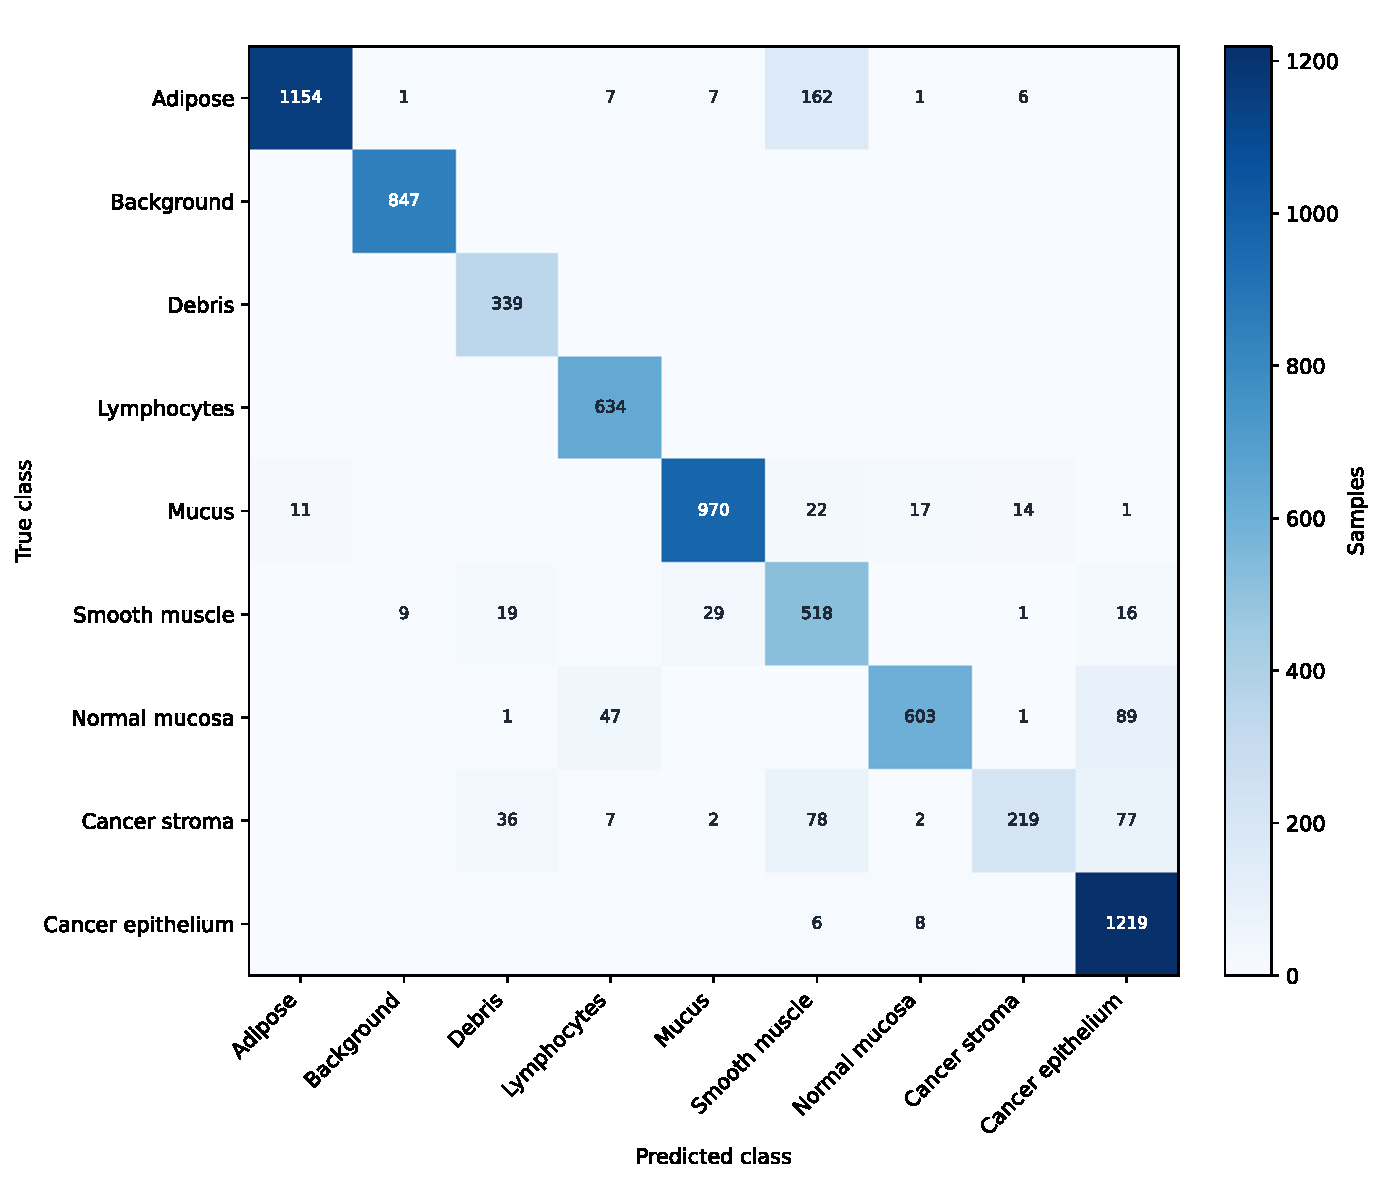
\includegraphics[width=\textwidth]{figures/baseline224_confusion_matrix}
    \end{column}
  \end{columns}
\end{frame}

\section{Diagnostics and Expert System}

\begin{frame}{Feature Visualization}
  \centering
  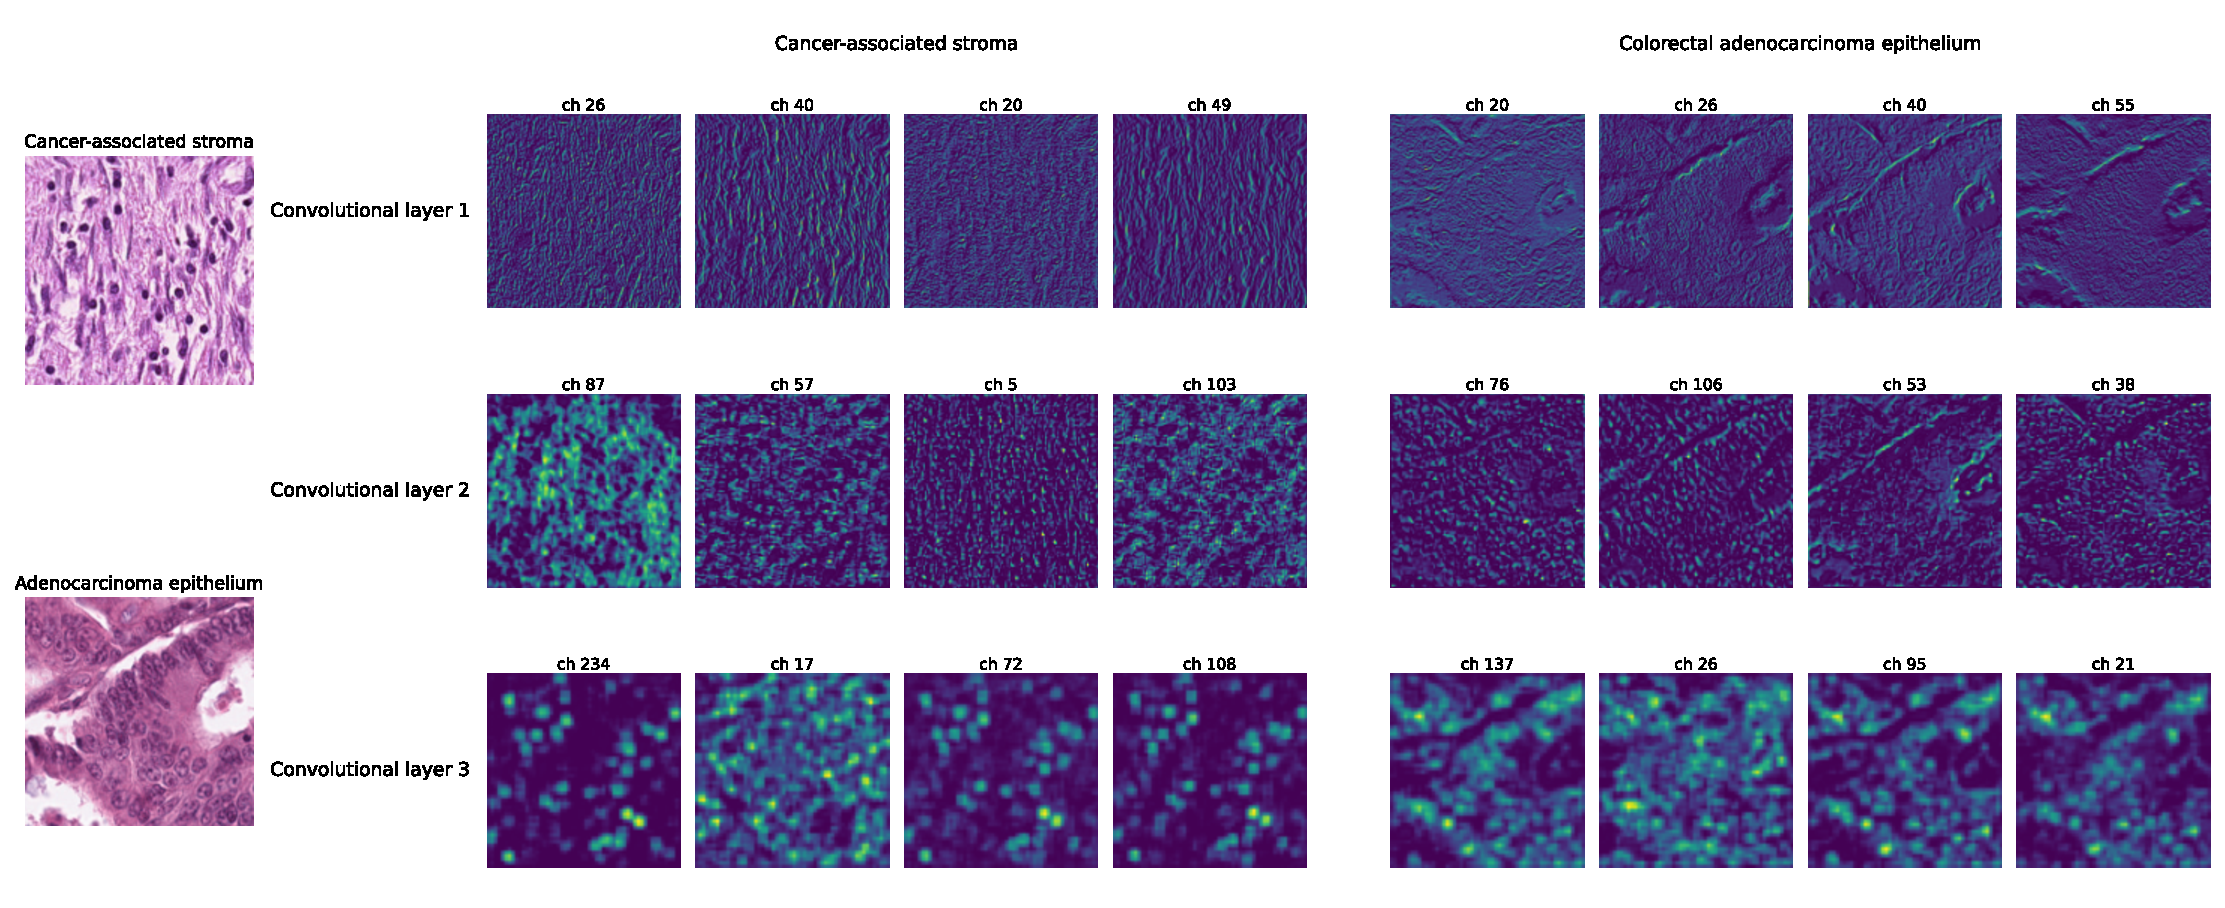
\includegraphics[width=0.90\textwidth]{figures/baseline224_cancer_feature_maps}
  \vspace{0.4em}
  \begin{itemize}
    \item Epithelium activations become more localized in deeper layers.
    \item Stroma activations stay more diffuse, suggesting a less stable representation.
  \end{itemize}
\end{frame}

\begin{frame}{Grad-CAM Visualization}
  \centering
  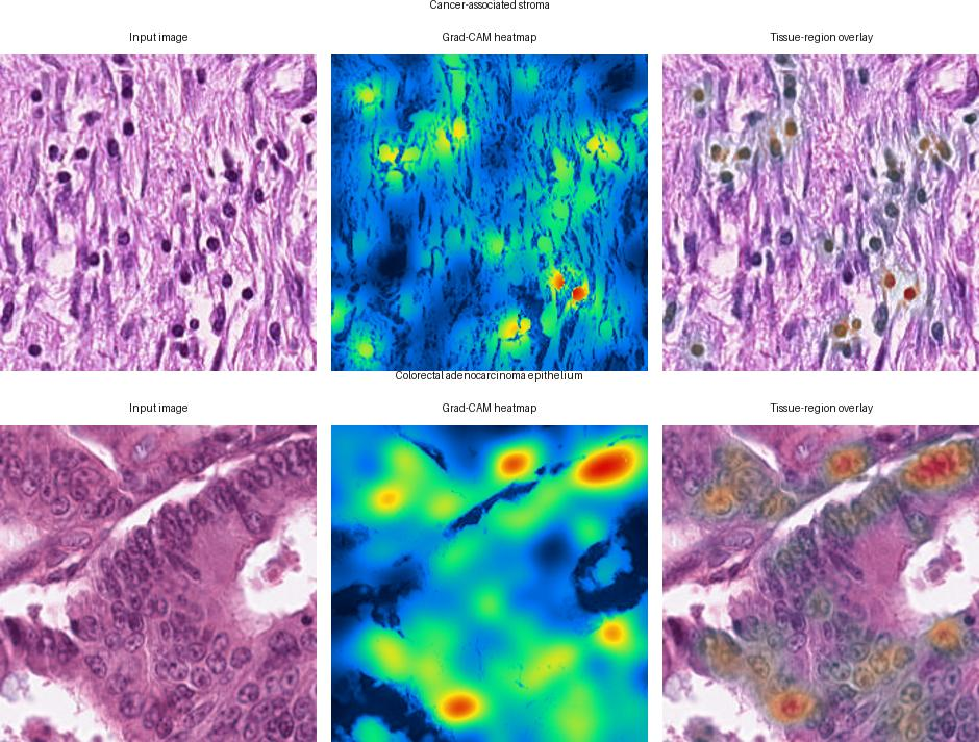
\includegraphics[height=0.86\textheight]{figures/baseline224_cancer_gradcam_vertical}
  % \begin{itemize}\small
  %   \item Stroma decisions are based on distributed texture-like regions.
  %   \item Epithelium decisions are more localized around dense epithelial structures.
  % \end{itemize}
\end{frame}

\begin{frame}{Prediction Confidences}
  \centering
  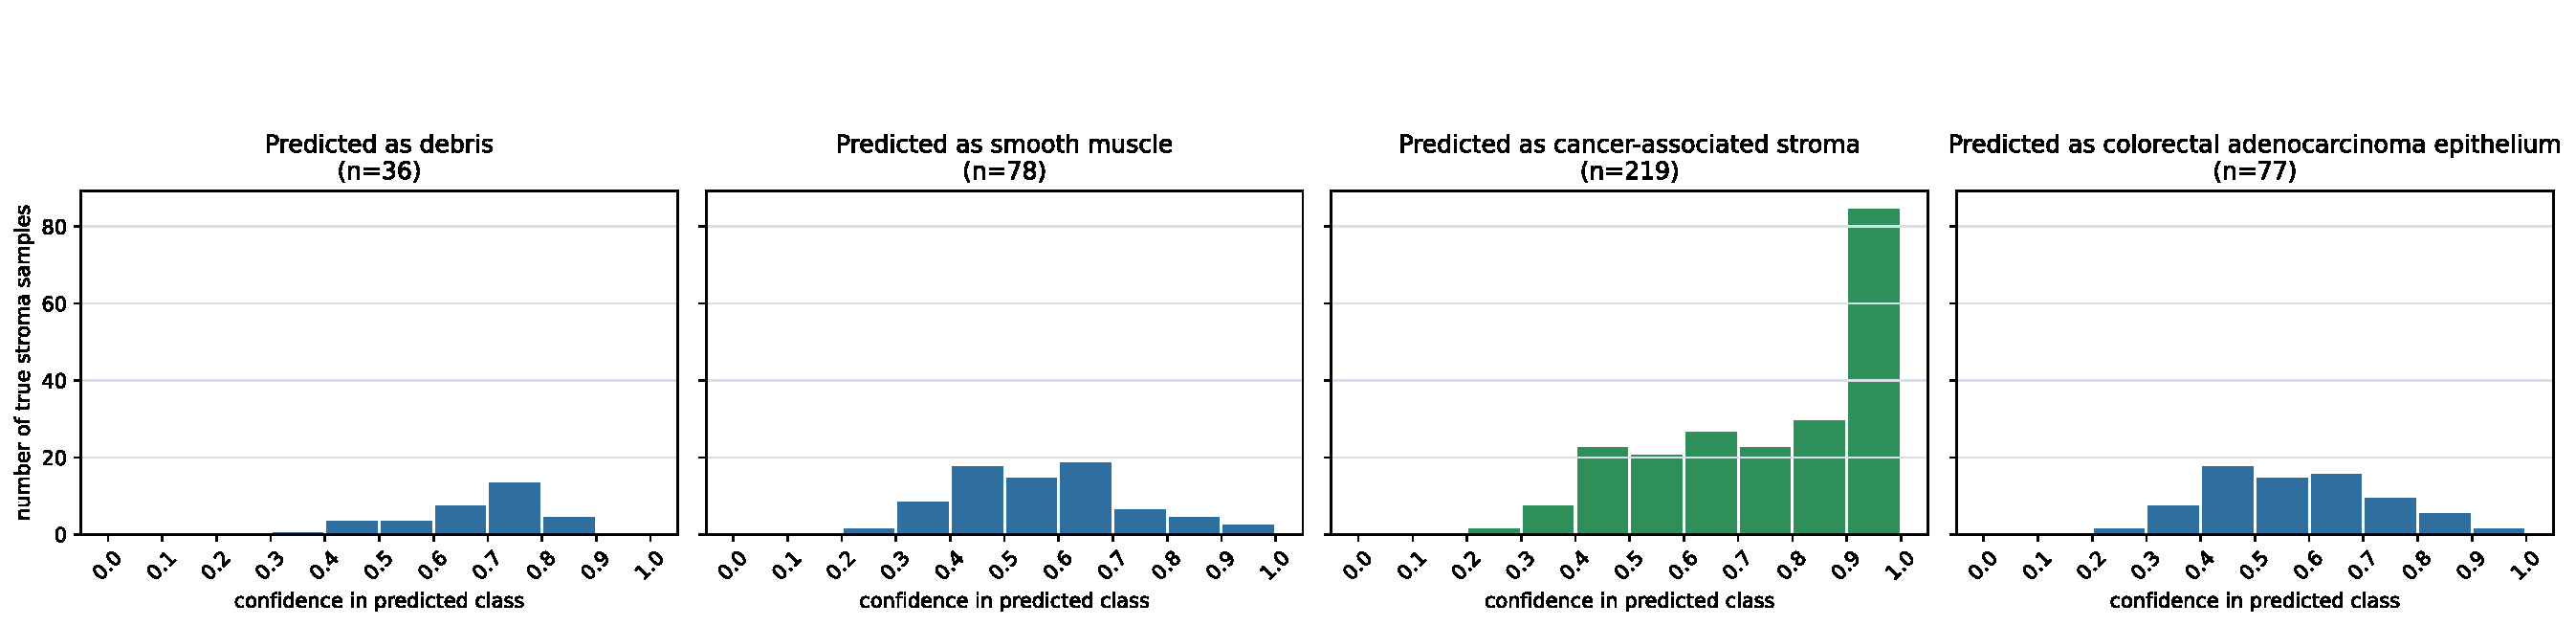
\includegraphics[width=0.94\textwidth]{figures/baseline224_stroma_confidence_distributions}
  \vspace{0.1em}
  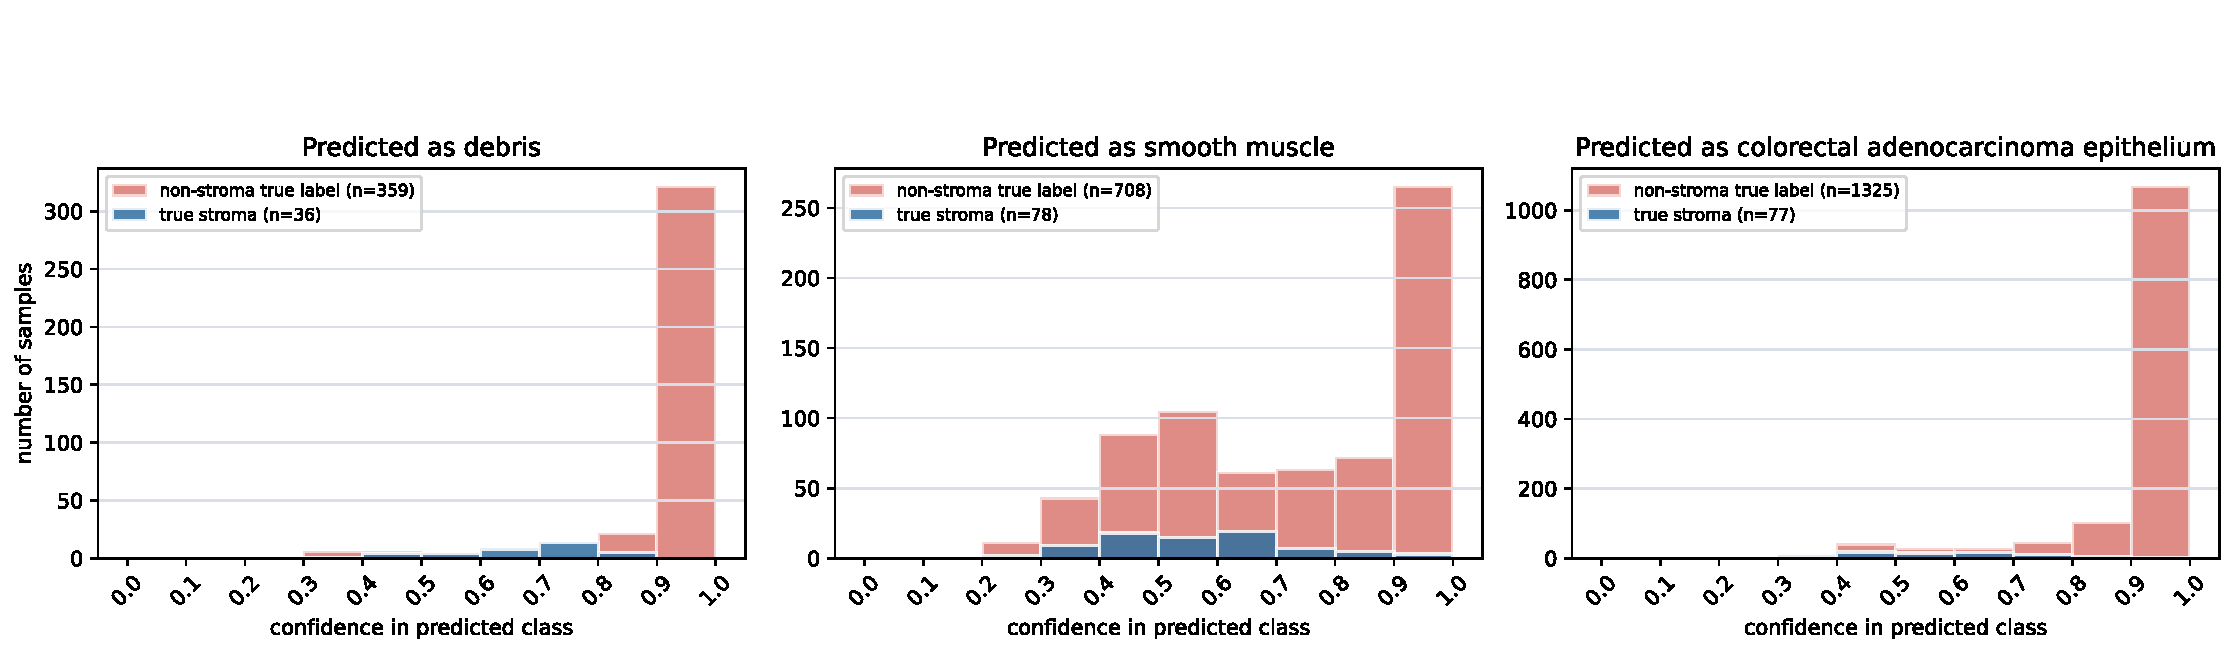
\includegraphics[width=0.94\textwidth]{figures/baseline224_stroma_nonstroma_confidence_comparison}
  % \begin{itemize}
  %   \item Many true stroma false negatives have only moderate confidence.
  %   \item High-confidence non-stroma predictions can usually be kept.
  %   \item Low-confidence predictions are candidates for specialist correction.
  % \end{itemize}
  % \begin{block}{Trigger rule}
  %   Consult an expert when the base model predicts a competing class with confidence below $\tau = 0.9$.
  % \end{block}
\end{frame}

\begin{frame}{Cancer Expert System}
  \centering
  \resizebox{0.96\textwidth}{!}{\begin{tikzpicture}[
    scale=0.7, transform shape,
    >=Latex,
    font=\small,
    box/.style={
        draw,
        rounded corners,
        thick,
        align=center,
        minimum height=1.1cm,
        minimum width=2.8cm,
        fill=blue!5
    },
    decision/.style={
        draw,
        diamond,
        thick,
        align=center,
        aspect=2.2,
        inner sep=1.2pt,
        fill=orange!8,
        text width=4.2cm
    },
    output/.style={
        draw,
        rounded corners,
        thick,
        align=center,
        minimum height=1.0cm,
        minimum width=2.1cm,
        fill=green!5
    },
    outer/.style={
        draw,
        rounded corners,
        very thick,
        inner xsep=10pt,
        inner ysep=10pt
    }
]

% --------------------------------------------------
% Nodes
% --------------------------------------------------

% Input centered between upper and lower paths
\node (input) at (-3.8,0) [box] {Sample $x$};

% Upper path
\node (base) at (0,1.4) [box, visible on=<2->] {Base model $\mathcal M_B$};
\node (baseout) at (3.0,1.4) [output, minimum width=1.3cm, visible on=<3->] {$\hat y_B$};
\node (decision) at (7.9,1.4) [decision, visible on=<4->]
{$\hat y_B \in \mathrm{Experts},$\\[2pt]
$p_B(\hat y_B \mid x) < \tau$};

\node (finalbase) at (13.3,1.4) [output, minimum width=2.3cm, visible on=<5->]
{$\hat y = \hat y_B$};

% Lower path
\node (expert) at (7.9,-1.4) [box, minimum width=2.9cm, visible on=<6->]
{Expert $\mathcal M_E$};

\node (finalexpert) at (13.3,-1.4) [output, minimum width=2.3cm, visible on=<7->]
{$\hat y = \hat y_E$};

% Final output outside the system box
\node (final) at (16.7,0) [output, minimum width=1.4cm, visible on=<8->]
{$\hat y$};

% --------------------------------------------------
% Helper coordinates
% --------------------------------------------------

\coordinate (inbranch) at (-1.8,0);
\coordinate (merge) at (14.8,0);

% --------------------------------------------------
% Arrows
% --------------------------------------------------

% Sample branching to both paths
\draw[-, thick, visible on=<2->] (input.east) -- (inbranch);
\draw[->, thick, visible on=<2->] (inbranch) |- (base.west);
\draw[->, thick, visible on=<6->] (inbranch) |- (expert.west);

% Main upper path
\draw[->, thick, visible on=<3->] (base) -- (baseout);
\draw[->, thick, visible on=<4->] (baseout) -- (decision);

% Decision branches
\draw[->, thick, visible on=<5->] (decision) -- node[above] {no} (finalbase);
\draw[->, thick, visible on=<6->] (decision) -- node[right] {yes} (expert);

% Expert output
\draw[->, thick, visible on=<7->] (expert) -- (finalexpert);

% Merge both internal outputs into final output
\draw[thick, visible on=<8->] (finalbase.east) -| (merge);
\draw[thick, visible on=<8->] (finalexpert.east) -| (merge);
\draw[->, thick, visible on=<8->] (merge) -- (final.west);

% --------------------------------------------------
% Outer system box
% --------------------------------------------------

\node[outer, fit=(base)(baseout)(decision)(expert)(finalbase)(finalexpert), visible on=<2->] (system) {};
\node[anchor=south west, font=\bfseries, visible on=<2->] at (system.north west)
{Cancer Expert};

\end{tikzpicture}
}
\end{frame}

\section{Results}

\begin{frame}{Confusion Matrix Comparison}
  \centering
  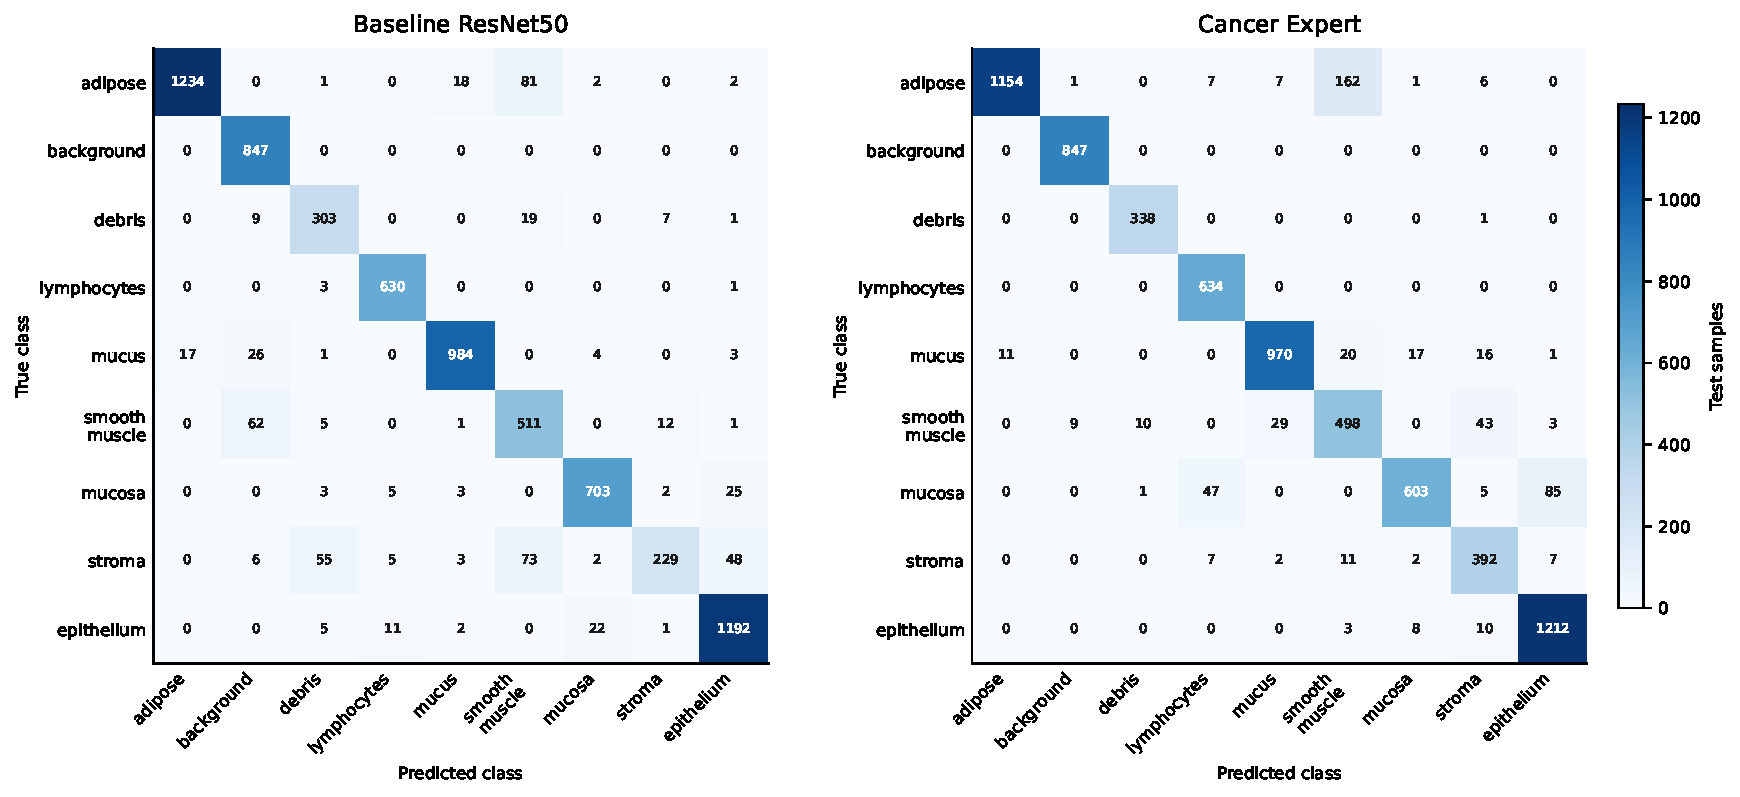
\includegraphics[width=0.82\textwidth]{figures/resnet50_cancer_expert_confusion_matrix_comparison}
  \vspace{0.2em}
  \begin{itemize}
    \item Correct stroma predictions increase from 229 to 392 out of 421.
    \item Stroma misclassified as debris, smooth muscle, and epithelium is strongly reduced.
  \end{itemize}
\end{frame}

\begin{frame}{Metric Comparison}
  \centering
  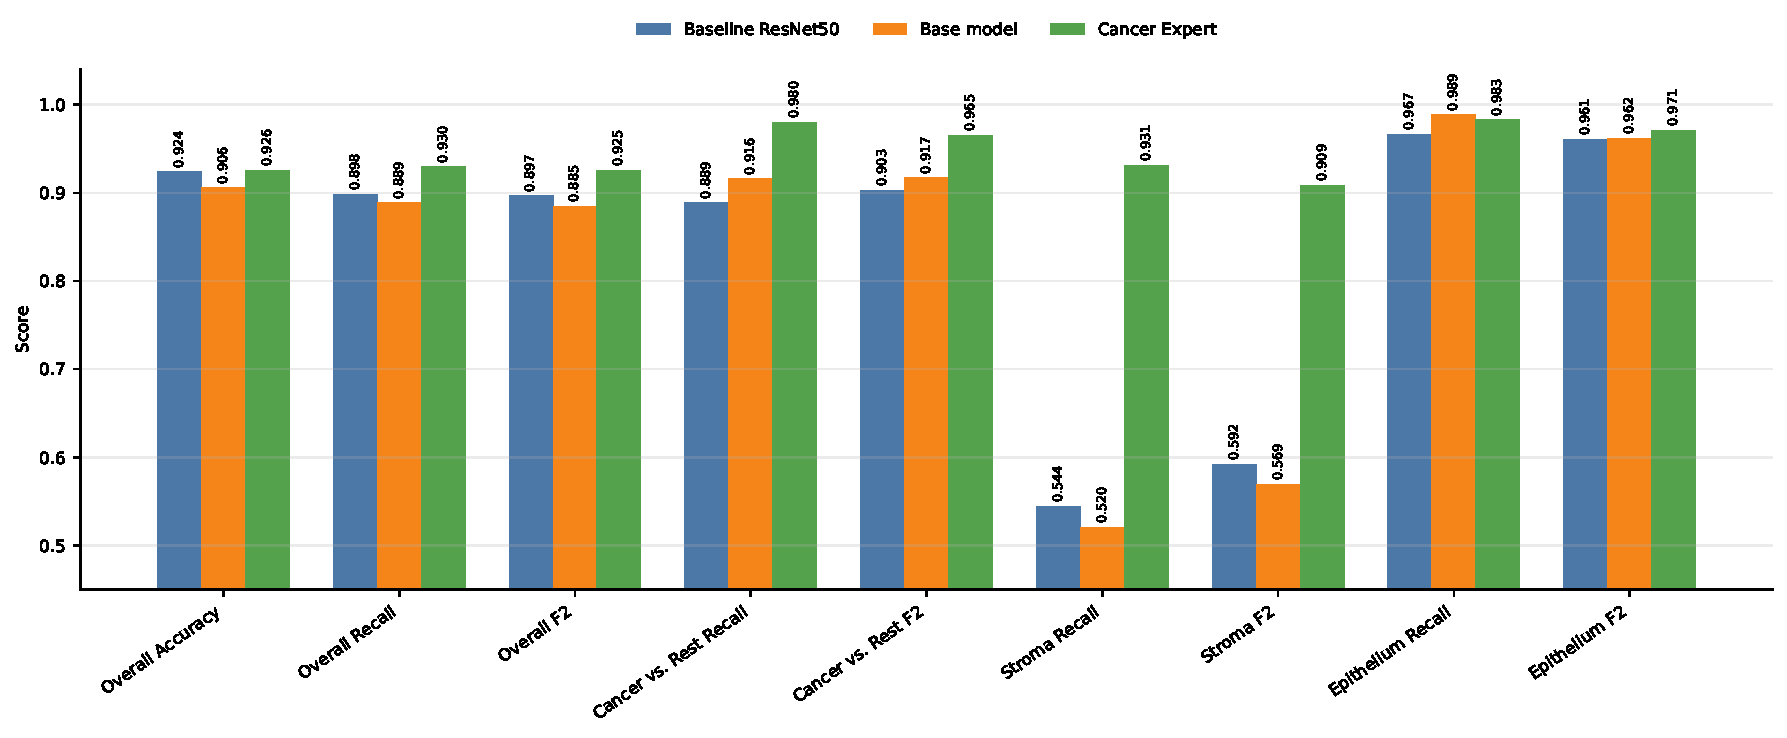
\includegraphics[width=0.98\textwidth]{figures/results_metric_comparison}
\end{frame}

\begin{frame}{Main Quantitative Improvements}
  \begin{columns}[T,onlytextwidth]
    \begin{column}{0.48\textwidth}
      \begin{block}{Compared with the base model}
        \begin{itemize}
          \item Stroma recall: $0.520 \rightarrow 0.931$.
          \item Stroma $F_2$: $0.569 \rightarrow 0.909$.
          \item Cancer-vs-rest recall: $0.916 \rightarrow 0.980$.
          \item Cancer-vs-rest $F_2$: $0.917 \rightarrow 0.965$.
        \end{itemize}
      \end{block}
    \end{column}
    \begin{column}{0.48\textwidth}
      \begin{block}{Trade-off}
        Epithelium recall decreases slightly, but mainly because some epithelium samples are reassigned to stroma.
      \end{block}
      \begin{block}{Aggregate result}
        Overall accuracy improves to $0.926$ and macro recall to $0.930$.
      \end{block}
    \end{column}
  \end{columns}
\end{frame}

\begin{frame}{Comparison to ResNet-50}
  \begin{itemize}
    \item ResNet-50 remains a strong external benchmark.
    \item The Cancer Expert achieves the best target metrics:
      \begin{itemize}
        \item overall accuracy,
        \item overall recall and $F_2$,
        \item cancer-vs-rest recall and $F_2$,
        \item stroma recall and stroma $F_2$.
      \end{itemize}
    \item The largest difference is stroma:
      \begin{itemize}
        \item ResNet-50 stroma recall: $0.544$.
        \item Cancer Expert stroma recall: $0.931$.
      \end{itemize}
  \end{itemize}
\end{frame}

\section{Conclusion}

\begin{frame}{Conclusion}
  \begin{itemize}
    \item The base CNN is a useful general classifier but has a clear class-specific weakness.
    \item Stroma false negatives concentrate in a small number of competing classes.
    \item Confidence distributions make it possible to trigger correction selectively.
    \item Binary expert classifiers substantially improve recall-oriented cancer metrics.
  \end{itemize}
  \begin{block}{Takeaway}
    Targeted expert correction can improve clinically relevant recall without sacrificing overall performance.
  \end{block}
\end{frame}

\begin{frame}{Limitations and Future Work}
  \begin{itemize}
    \item The expert system is evaluated on PathMNIST only.
    \item Expert thresholds are manually selected and should be tuned more systematically.
    \item Hyperparameters for the basemodel and expert classifiers are not optimized.
    \item The approach increases pipeline complexity compared with a single classifier.
    \item Real-world applications use more sophisticated models, such as vision transformers.
  \end{itemize}
\end{frame}

\begin{frame}{Thank You}
  \centering
  \Large
  Any Questions?
\end{frame}


\end{document}
